\section{Kiến thức nền tảng}
Trước khi đi vào nghiên cứu bài đề cương luận văn này, một số kiến thức nền tảng cần được nhắc lại như sau.
\subsection{Các kiến thức toán cơ bản}
\subsubsection{Phép nhân tích chập ma trận (convolution)}\label{subsec:convlop}

Nhân tích chập là phép toán quan trọng trong Xử lý ảnh số và thị giác máy tính, là công cụ chủ yếu để thực hiện các phép tính toán trên ảnh như đạo hàm ảnh, làm trơn ảnh hay trích xuất cạnh.

Trong toán học, tích chập là phép toán trên hai hàm f và g, tạo ra hàm thứ ba là hàm (f*g). Công thức phép tích chập trên miền liên tục một chiều như sau:

\begin{equation}
    (f*g)(t) \triangleq \displaystyle \int_{-\infty}^{\infty}f(\tau)g(t-\tau)d\tau
\end{equation}

Đối với trong Xử  lý ảnh, phép tích chập được tính trên miền không gian hai chiều, rời rạc. Công thức tính tích chập trên ảnh f và bộ lọc k (kích thước mxn) tại điểm ảnh vị trí (x,y) với giả sử chỉ số trên bộ lọc được đánh số hàng từ -m/2 -> m/2 và chỉ số cột từ -n/2 -> n/2:

\begin{equation}
    (k*f)(x,y) \triangleq \displaystyle \sum_{u=-m/2}^{m/2}\displaystyle \sum_{v=-n/2}^{n/2}k(u,v)f(x-u,y-v)
\end{equation}

Một phép toán tương tự covolution nhưng không xoay bộ lọc như trên, gọi là correlation (hình \ref {fig:correlation}), công thức như sau:
\begin{equation}
    (k*f)(x,y) \triangleq \displaystyle \sum_{u=-m/2}^{m/2}\displaystyle \sum_{v=-n/2}^{n/2}k(u,v)f(x+u,y+v)
\end{equation}

\begin{figure}[!htp]
    \begin{center}
        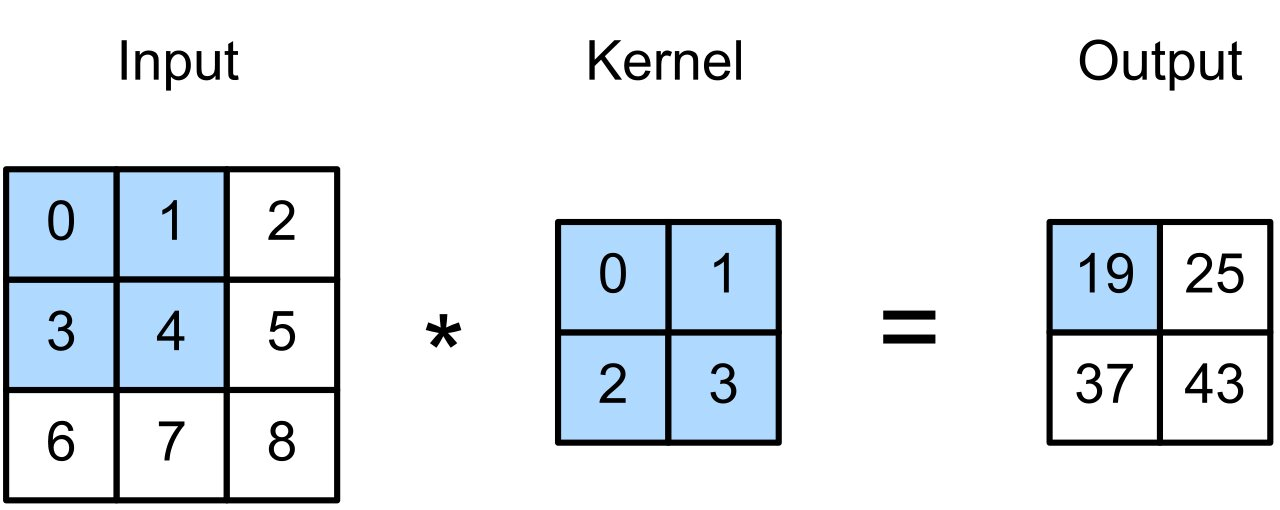
\includegraphics[width=\linewidth]{asset/image/correlation.jpg}
        \caption{Phép correlation.}
        \label{fig:correlation}
    \end{center}
\end{figure}

%chưa nhắc tới strike hay padding gì cả

%graph
\subsubsection{Đồ thị (graph)}

Đồ thị là cấu trúc rời rạc bao gồm các cạnh và các đỉnh được kết nối với nhau thông qua các cạnh đó. Có nhiều loại đồ thị khác nhau, phụ thuộc vào việc có hay không các chiều (direction) của các cạnh, một hay nhiều cạnh cùng kết nối một cặp đỉnh và có chu kì hay không \cite{rosen2012discrete}.

\textbf{Định nghĩa:}

Một đồ thị G=(V,E) bao gồm V, một tập không rỗng các đỉnh (hay nodes) và E, một tập các cạnh. Mỗi cạnh có một hoặc hai đỉnh liên kết với nó, gọi là endpoints. Một cạnh sẽ kết nối các endpoints của nó \cite{rosen2012discrete}.

\textbf{Phân loại đồ thị:}

Đồ thị được chia thành nhiều loại dựa vào ba tiêu chí sau:
\begin{enumerate}
    \item Đồ thị có hướng hoặc vô hướng.
    \item Đơn đồ thị hoặc đa đồ thị.
    \item Đồ thị có chu trình hoặc không có chu trình.
\end{enumerate}

Trong Đề cương luận văn này, loại đồ thị được tập trung chủ yếu là đồ thị đơn, vô hướng và không có chu trình. Sau đây ta đi vào cách xây dựng một graph model từ cấu trúc các khớp (joint), xương (bone) của các đối tượng người.

Đối với khung xương người, mỗi khớp sẽ được mô hình hóa thành một đỉnh trong đồ thị, giá trị chứa trong đỉnh là tọa độ của khớp đó trong khung hình (với điểm gốc được định nghĩa tùy vào mục đích bài toán). Mỗi cạnh biểu thị hai đỉnh tương quan với nhau, tức là tồn tại xương giữa hai khớp đó. Độ dài ngắn biểu thị độ xa gần của các khớp. Tùy mục đích mà việc chọn các khớp nào,  hay các xương nào để  mô hình hóa bài toán. Ví dụ với bài toán nhận diện cử chỉ tay, việc tập trung chi tiết các khớp xương ở tay sẽ rất có giá trị, trong khi các khớp xương ở chân và các bộ phận khác sẽ không đóng góp nhiều, do đó không cần định nghĩa trong bài toán.

\begin{figure}[!htp]
    \begin{center}
        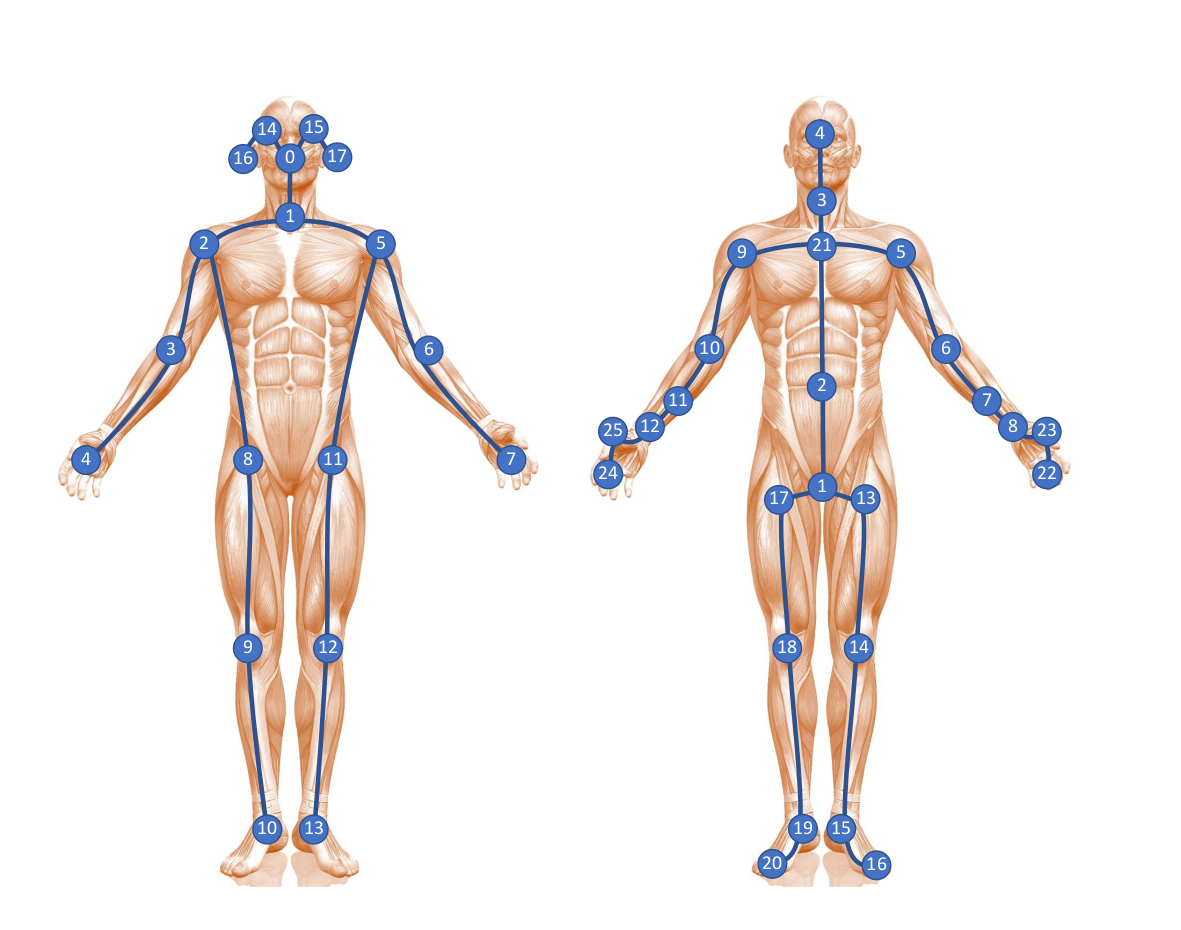
\includegraphics[width=\linewidth]{asset/image/skeleton.png}
        \caption{Graph model cho khung xương người (tham khảo \cite{shi2020skeleton}). }
        \label{fig:skeleton}
    \end{center}
\end{figure}

Trong mô hình thực tế nhóm đang nghiên cứu, tức với mục tiêu nhận diện nhiều loại hành vi của con người, ngoài các cạnh biểu thị các xương sẵn có như hình \ref{fig:skeleton}, nhóm còn định nghĩa thêm các cạnh biểu thị sự tương quan giữa hai đỉnh mà nhóm cho là cần thiết cho mục tiêu bài toán, ví dụ các cạnh giữa hai khớp tay hay giữa khớp tay với khớp chân (hình \ref{fig:morebones}).

\begin{figure}[!htp]
    \begin{center}
        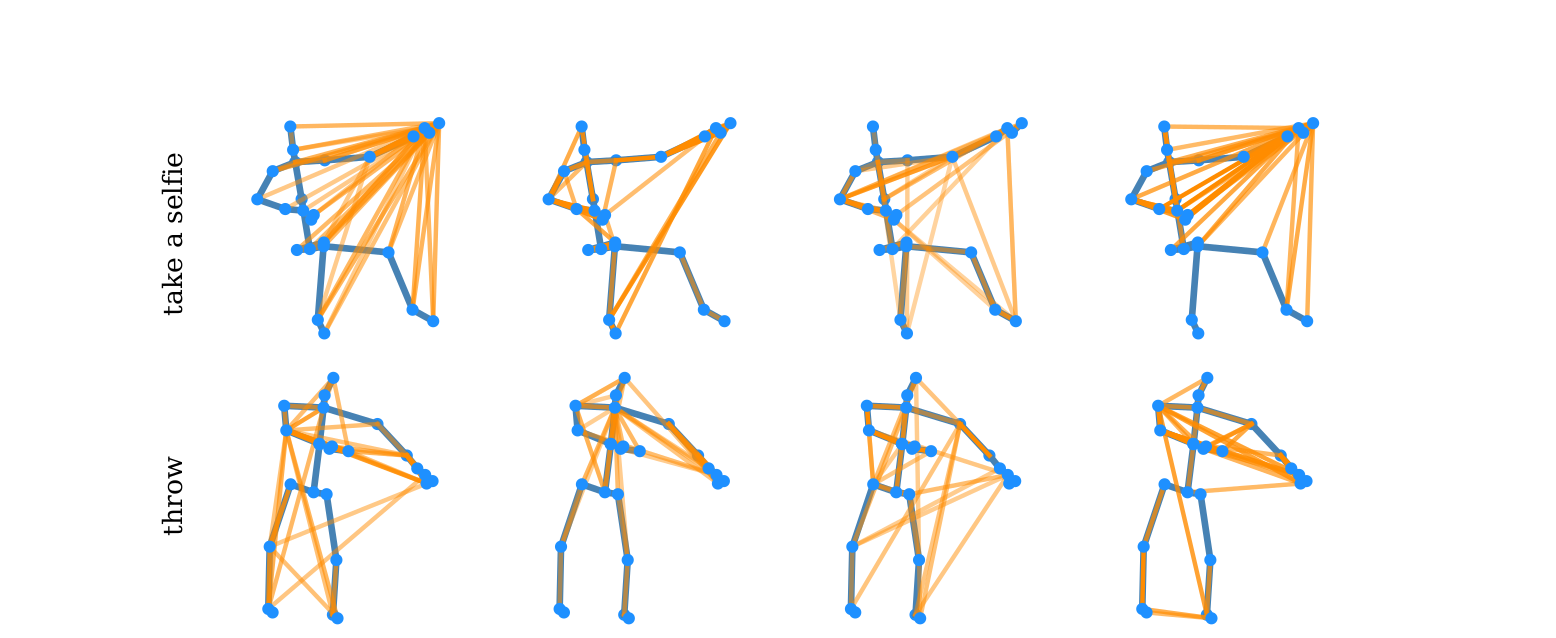
\includegraphics[width=\linewidth]{asset/image/morebones.png}
        \caption{Graph model cho khung xương người với các cạnh bổ sung (tham khảo \cite{shi2020skeleton}). }
        \label{fig:morebones}
    \end{center}
\end{figure}

\subsection{Các kiến thức cơ bản về  Trí tuệ nhân tạo, học máy và học sâu}
\subsubsection{Các kiến thức cơ bản}
%TODO: gradient descent, overfit, underfit, hội tụ, bias, variant, weight, model, loss function, .. tham khảo machinelearningcoban để tránh thiếu sót
%ANN co ban (duoc su dung trng bai: Batch norm, Convolution, resnet, activation: sigmoid, relu,..): embeđing, GCN 
\textbf{Gradient descent - back propagation}

Trong các bài toán tối ưu, việc sử dụng đạo hàm là phương pháp chủ yếu để tìm các điểm cực trị. Việc giải phương trình đạo hàm bằng không đưa ra một tập nghiệm mà tại đó ta chọn ra được các điểm cực trị cần tìm  một cách chính xác. Tuy nhiên với một số bài toán phức tạp, hay các bài toán bất khả vi thì việc giải phương trình đạo hàm bằng không là rất khó, thậm chí là không tồn tại nghiệm. Điều đó đặc biệt đúng trong ngữ cảnh máy học, việc tính chính xác điểm cực trị trong các mô hình học sâu gần như là bất khả thi. Một phương pháp thay thế  để đơn giản hóa việc này, tuy nhiên vẫn giữ được độ chính xác tương đối để đáp ứng nhu cầu bài toán được gọi là \textit{Gradient descent}.

% ******************************************************************************
\begin{figure}[!ht]
    % caption on side     
    \floatbox[{\capbeside\thisfloatsetup{capbesideposition={right,top},capbesidewidth=6cm}}]{figure}[\FBwidth]
    {\caption{
            Khảo sát sự biến thiên của một đa thức bậc hai (tham khảo \cite{tiep2018machine}).
        }
        \label{fig:grad}}
    { % figure here
        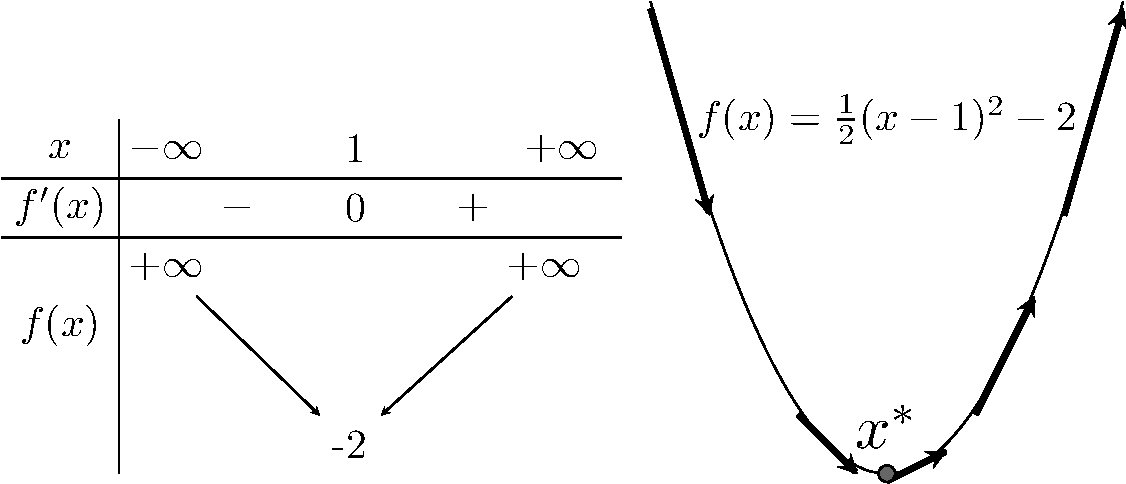
\includegraphics[width=.5\textwidth]{asset/pdf/gradient_descent.pdf}
    }
\end{figure}
% ********

Để  hiểu đươc ý tưởng của \textit{gradient descent}, ta đi vào nghiên cứu ứng dụng của phương pháp  để tìm điểm cực trị của hàm một biến. Xét hàm số $f(x) = \frac{1}{2}(x-1)^2 -2$ có độ thị như hình \ref{fig:grad}, mục tiêu là sử dụng gradient descent để đưa giá trị mà ta cho là nghiệm xấp xỉ $x_t$ về gần với nghiệm thực sự $x^*$. Ta khảo sát đạo hàm $f'(t)$ tại điểm $x_t$ như sau:

\begin{itemize}
    \item nếu $f'(t)>0$ tức $x_t$ lúc này đang ở bên phải của $x^*$, lúc này cần dời vị trí $x_t$ sang bên trái vị trí hiện tại.
    \item ngược lại nếu $f'(t)<0$ tức lúc này $x_t$ đang ở bên trái của $x^*$, và $x_t$ cần được dời về bên phải vị trí hiện tại.
\end{itemize}

Tổng hợp hai trường hợp trên, ta đều phải dời $x_t$ theo chiều ngược lại với giá trị đào hàm tại đó, điều này tương đương với công thức sau:

\begin{equation}
    x_(t+1) = x_t - \eta f'(t)
\end{equation}

Trong đó giá trị $\eta$ thường được gọi là \textit{tốc độ học (learning rate)}. Dấu trừ biểu thị cho việc dời $x_t$ ngược chiều với giá trị đạo hàm. (tham khảo \cite{tiep2018machine})

Trong học máy, Gradient descent ứng dụng cho việc cập nhật các tham số giữa các layer của mạng. Việc cập nhật các tham số này (trình bày ở mục \ref{subsubsec:ann}) sẽ được thực thi từ layer cuối cùng trở về trước, do việc tính đạo hàm phải bắt đầu theo thứ tự đó. Quá trình cập nhật tham số  này được gọi là lan truyền ngược (back propagation).

\textbf{Overfitting}

Trong học máy, để một mô hình (model) có thể hoạt động được, ta cần một quá trình giúp mô hình thu nạp kiến thức cần thiết cho việc hoạt động của mô hình, đó được gọi là quá trình học. Quá trình học giúp mô hình có thể cải thiện mức độ khớp (fit) giữa input và output trong tập dữ liệu huấn luyện (training set). Nhưng việc một mô hình có mức độ khớp vượt quá mức cần thiết (overfit) sẽ mang lại hiểu quả không cao, vì lúc này tính tổng quát của mô hình bị giảm đáng kể. Khi một mô hình bị overfit, các tham số của mô hình có xu hướng mô tả chính xác tập dữ liệu huấn luyện nhưng không có khả năng đưa ra phán đoán tốt cho những dữ liệu input mà nó chưa được thấy, đây là điều cần tránh trong học máy.

Trái với hiện tượng này là underfitting, đây là trường hợp mà mô hình chưa được thu nạp đủ kiến thức cho việc đưa ra phán đoán, do đó dẫn tới hiện tượng phán đoán sai trên ngay cả tập dữ liệu huấn luyện và dữ liệu kiểm thử.

Một số phương pháp để giảm hiện tượng overfitting có thể kể tới là validation (hoặc cross-validation nếu tập dữ liệu hạn chế), regularization và early stopping (được trình bày trong tham khảo \cite{tiep2018machine}).

\textbf{Variance - bias}

Trong học máy, hai khái niệm quan trọng cần biết để giúp việc điều chỉnh mô hình tốt hơn đó là \textit{bias} và \textit{variance}. Hai khái niệm này còn được gọi là sai số dự đoán (prediction errors). Để đơn giản, lấy ví dụ trong bài toán Hồi quy tuyến tính (linear regression), giả sử ta có tập dữ liệu huấn luyện với mối quan hệ input, output như sau:
\begin{equation}
    Y = f(X) + e
\end{equation}

Trong đó e là phần sai số (error term), thông thường tuân theo một phân phối với giá trị mean bằng không ($E(e)=0$), X,Y là input và output tương ứng trong tập dữ liệu huấn luyện $\tau$.
Xét bài toán hồi quy tuyến tính nhằm tìm xấp xỉ $\widehat{f}(X)$ của $f(X)$. Hàm lỗi được chọn là trung bình bình phương (mean square error) như sau:

\begin{subequations}\label{eqn}
    \begin{align*}
        Error(\widehat{f},\tau) & = E(Y- \widehat{f}(X))^2)                      \\
                                & = E(f(X)+e- \widehat{f}(X))^2) \tag{\ref{eqn}}
    \end{align*}
\end{subequations}

Lúc này giá trị Bias và Variance lần lượt:

\begin{equation}\label{bias}
    Bias(\widehat{f},\tau) = E(  (f(X) - E(   \widehat{f}(X)))^2 )
\end{equation}
\begin{equation}\label{var}
    Variance(\widehat{f},\tau) = E(  (E(\widehat{f}(X)) - \widehat{f}(X))^2 )
\end{equation}

Thay các giá trị tương ứng từ \ref{bias} và \ref{var} vào \ref{eqn} ta được:

\begin{equation}
    Error(\widehat{f},\tau) = Bias(\widehat{f},\tau) +  Variance(\widehat{f},\tau) + E(e^2)
\end{equation}

Trong đó $E(e^2)$ là lượng không thay đổi được, từ đó cho thấy giá trị bias và variance ảnh hưởng trực tiếp tới sai số dự đoán của mô hình.

Một cách trực quan có thể xem hình \ref{fig:bias} sau:
\begin{figure}[!ht]
    \begin{center}
        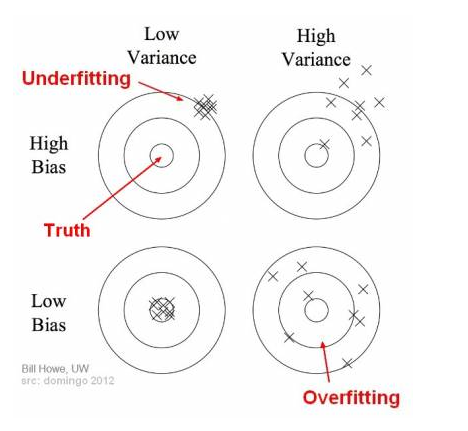
\includegraphics[width=\linewidth]{asset/image/bias.png}
        \caption{Minh họa trực quan bias và variance (tham khảo \cite{breiman1996bias}). }
        \label{fig:bias}
    \end{center}
\end{figure}

Một vấn đề khi cố gắng giảm bias thì variance sẽ tăng, và ngược lại, vấn đề này gọi là variance-bias tradeoff. Trong khi xây dựng mô hình, cần lựa chọn đánh đổi phù hợp để chọn được mô hình tốt nhất cho bài toán.

\textbf{Loss function (cost function)} (tham khảo \cite{tiep2018machine})

Để một mô hình học máy có thể cải thiện theo xu hướng mong muốn, cần có một chỉ dẫn để việc cập nhật các tham số theo hướng có tốt hơn. Việc chỉ dẫn này được cụ thể hóa bằng một hàm số gọi là hàm mất mát (loss function hoặc cost function). Thông thường khi hàm mất mát đạt giá trị càng thấp thì mô hình có khả năng dự đoán càng chính xác. Nói cách khác, việc xây dựng mô hình cũng giống như việc tối ưu một hàm số, quá trình tối ưu đó, trong học máy gọi là \textit{learning}. Ký hiệu của hàm mất mát $J(\theta)$, khi đó tham số cần tìm là:

\begin{equation}
    \theta ^* = \underset{\theta}{\operatorname{argmin(J(\theta))}}
\end{equation}


\textbf{Mạng nơ-ron nhân tạo (artificial neural network)} \label{subsubsec:ann} (tham khảo \cite{abraham2005artificial})

Mạng nơ-ron nhân tạo là một lĩnh vực nghiên cứu trong học máy, có nhiệm vụ cố gắng mô phỏng cách mà não bộ con người phân tích và xử lý thông tin. Sự ra đời của kiến trúc này đã giúp giải được các bài toán khó và phức tạp đối con người hay các phương pháp thống kê thông thường. Đây là kiến trúc có khả năng tự học và cải thiện khả năng để đưa ra kết quả tốt hơn khi nhiều dữ liệu được cung cấp cho mạng. Mô phỏng kiến trúc một ANN đơn giản như hình \ref{fig:anniamg}.

\begin{figure}[!htp]
    \begin{center}
        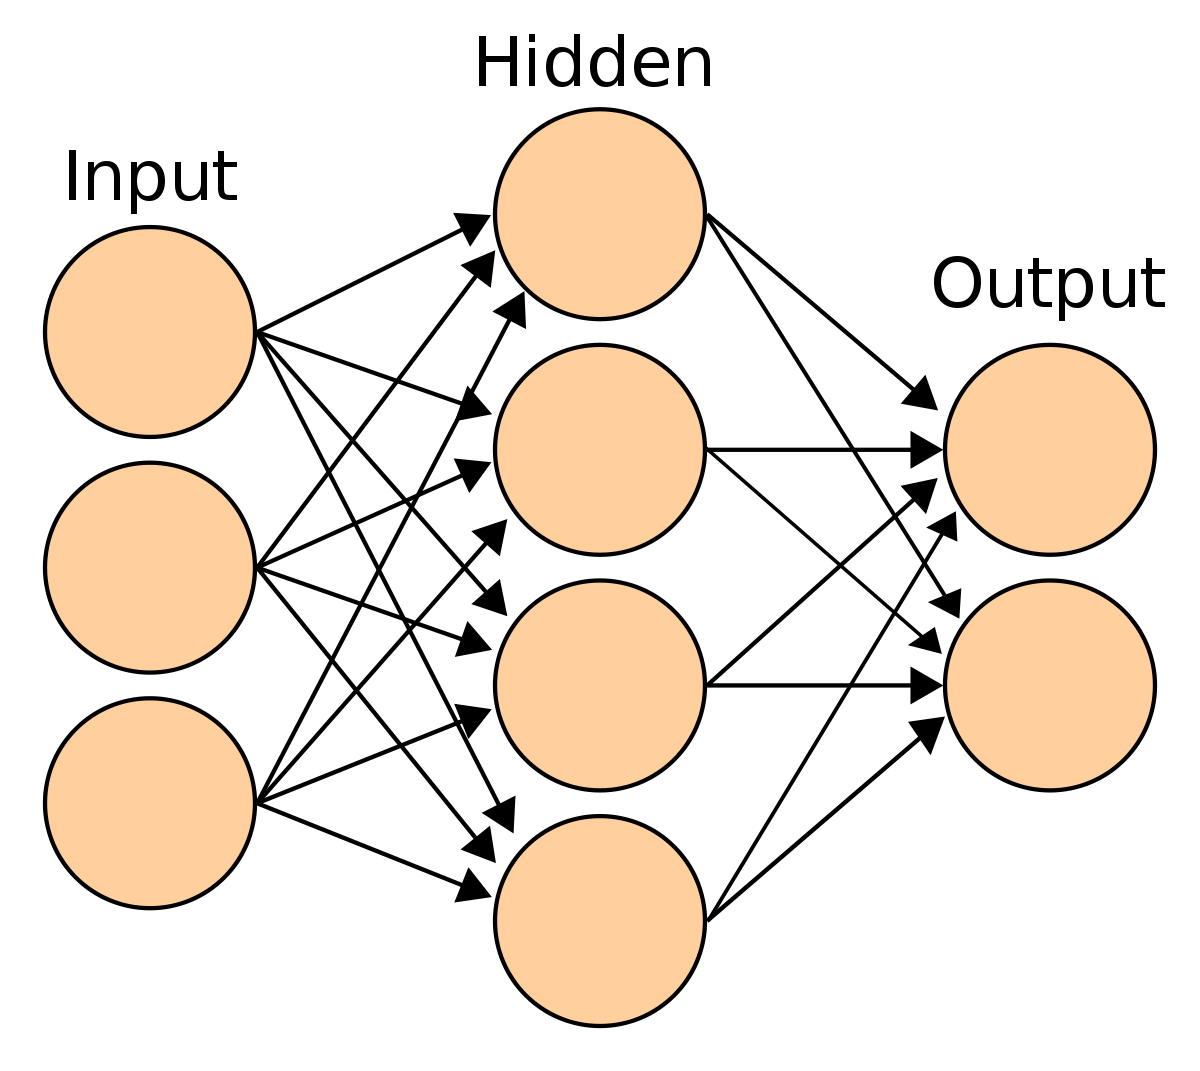
\includegraphics[scale=0.2]{asset/image/anniamg.png}
        \caption{Kiến trúc một ANN đơn giản.}
        \label{fig:anniamg}
    \end{center}
\end{figure}

Trong đề cương luận văn này, một số loại mạng nơ-ron nhân tạo được ứng dụng, cụ thể là: mạng tích chập thông thường (Convolutional neural network), mạng tích chập đồ thị (Graph convolutional network) với các layer khác được thêm vào hay bớt đi để phù hợp với mục đích bài toán.

Sau đây sẽ đi qua một vài loại layer quan trọng được sử dụng trong bài toán.
\begin{itemize}
    \item Convolutional layer:

          Trong xử lý ảnh, thông thường thuộc tính toàn cục (global) của bức hình không chứa nhiều giá trị bằng thuộc tính cục bộ (local). Vì vậy Kunihiko Fukushima đã đưa ra một loại layer rất phổ biến ngày nay với tên gọi Convolutional  layer(tham khảo \cite{fukushima1988neocognitron}).

          Convolutional layer sử dụng phép toán tích chập ma trận (được trình bày ở mục \ref{subsec:convlop}) để rút trích đặc trưng cục bộ của bức hình. Phương pháp này đem lại hiệu quả đáng kể trong xử lý hình ảnh với khả năng khai thác đặc tính không gian của bức hình.

          % \item Graph convolution layer
          % \item 
          % \item BatchNorm layer
    \item Resnet layer (tham khảo \cite{he2016deep})

          Trong mô hình học sâu (deep learning), việc cập nhật các tham số mô hình gặp một vấn đề được gọi là \textit{vanishing gradients}. Nguyên nhân do kiến trúc mô hình nhiều layer, nên khi tính đạo hàm tới các layer thấp (các layer ban đầu), gradients có xu hướng nhỏ dần, điều này làm cho các lớp này không còn khả năng học tốt nữa. Đây là sự ra đời của mạng ResNet, giúp cho việc học của các mô hình học sâu được hiệu quả và ổn định hơn.

          Mạng RestNet khá tương tự các mạng khác với các layer convolution, pooling, activation, fully-connected, chỉ khác ở chỗ có các đường dư thừa (residual block) nối tắt qua một vài layer (hình \ref{fig:restnet}). Kết quả thực nghiệm đã cho thấy mô hình học sâu kết hợp restnet có thể cải thiện khi độ chính xác tăng nhưng không tăng thêm độ phức tạp mô hình (tham khảo \cite{he2016deep}).

          \begin{figure}[t]
              \begin{center}
                  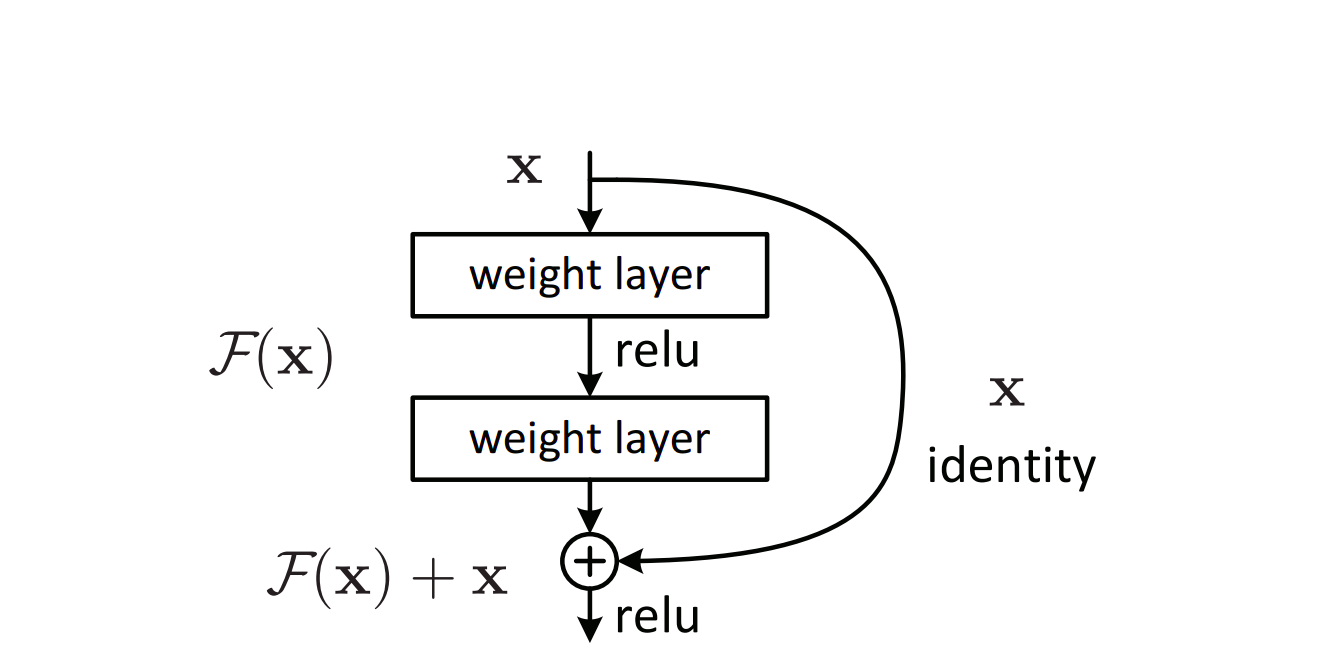
\includegraphics[scale=0.2]{asset/image/restnet.png}
                  \caption{Một Residual block. }
                  \label{fig:restnet}
              \end{center}
          \end{figure}
    \item Activation function: sigmoid, relu.

          Trong hệ thống thần kinh người, các xung thần kinh được truyền giữa các nơ-ron thông qua các axon. Để  mô phỏng quá trình truyền xung thần kinh của người qua axon theo một tỷ lệ, người ta dùng hàm kích hoạt (activation function). Trong một mạng nơ-ron nhân tạo, hàm kích hoạt đóng vai trò là thành phần phi tuyến giúp cho mô hình có khả năng biểu diễn được một hàm phức tạp giữa input và output của mạng.

          Hai loại hàm kích hoạt được sử dụng chủ yếu trong đề cương luận văn này là sigmoid (hình \ref{fig:sigmoid}) và relu (hình \ref{fig:relu}).
          % phân tích ưu nhược điểm từng hàm: https://aicurious.io/posts/2019-09-23-cac-ham-kich-hoat-activation-function-trong-neural-networks/
          
          Hàm sigmoid:
          \begin{equation}
              \sigma(x) = \frac{1}{1+e^{-x}}
          \end{equation}

          \begin{figure}[t]
              \begin{center}
                  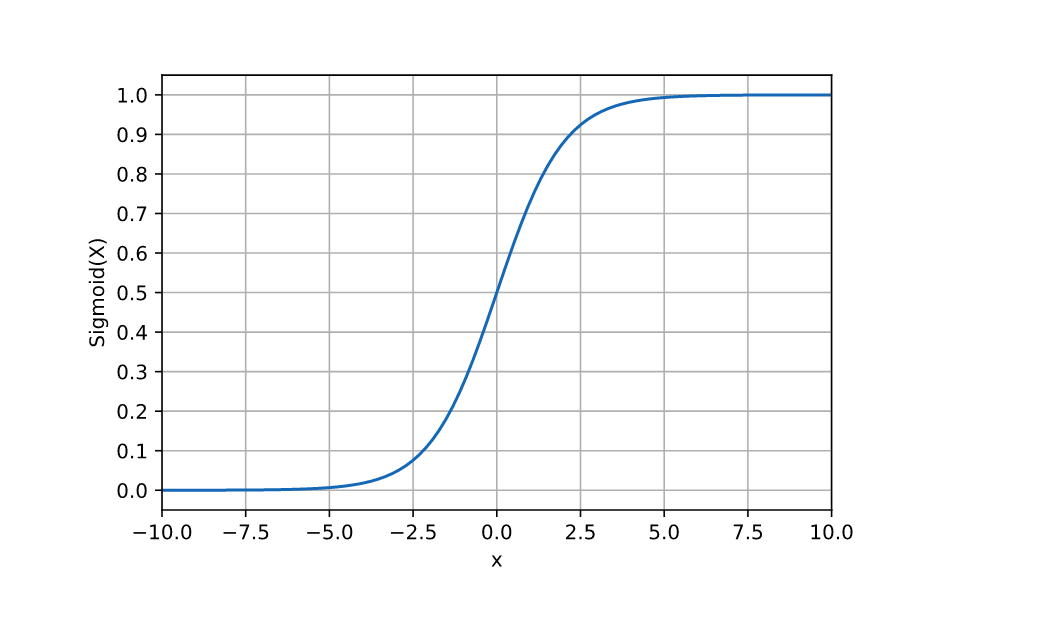
\includegraphics[scale=0.2]{asset/image/sigmoid.png}
                  \caption{Hàm sigmoid. }
                  \label{fig:sigmoid}
              \end{center}
          \end{figure}


          Hàm Relu:
          \begin{equation}
              f(x) = max(0,x)
          \end{equation}

          \begin{figure}[t]
              \begin{center}
                  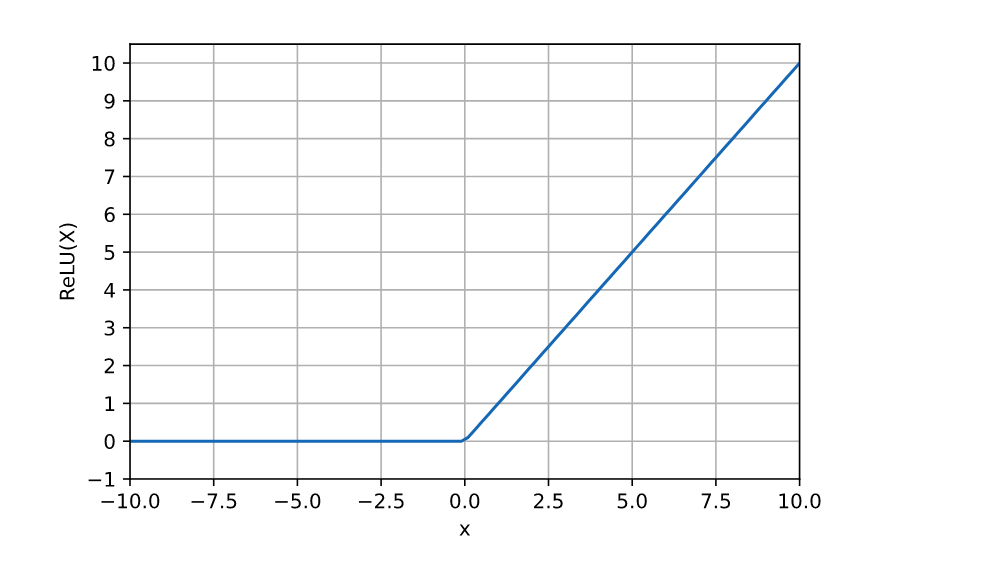
\includegraphics[scale=0.2]{asset/image/relu.png}
                  \caption{Hàm Relu. }
                  \label{fig:relu}
              \end{center}
          \end{figure}


\end{itemize}

\textbf{Kỹ thuật nhúng -  embedding}

% An embedding is a mapping of a discrete — categorical — variable to a vector of continuous numbers. In the context of neural networks, embeddings are low-dimensional, learned continuous vector representations of discrete variables. Neural network embeddings are useful because they can reduce the dimensionality of categorical variables and meaningfully represent categories in the transformed space.
Nhúng (embedding) là một khái niệm phổ biến trong máy học, thực chất của việc này là đưa một biến rời rạc về dạng một vector với giá trị liên tục. Kết quả của việc nhúng thường là giảm chiều của dữ liệu hoặc đưa dữ liệu về dạng có ý nghĩa hơn trong miền không gian mới.

% Neural network embeddings have 3 primary purposes:
% Finding nearest neighbors in the embedding space. These can be used to make recommendations based on user interests or cluster categories.
% As input to a machine learning model for a supervised task.
% For visualization of concepts and relations between categories.

Có ba mục đích chính của việc nhúng dữ liệu trong Neural network đó là:
\begin{enumerate}
    \item Tìm các hàng xóm (neighbors) lân cận trong không gian nhúng. Thường được sử dụng trong các bài toán gợi ý (recommendation) cho các dữ liệu về sở thích người dùng.
    \item Được sử dụng như là input cho một mô hình machine learning trong các bài toán học giám sát.
    \item Được sử dụng cho mục đích trực quan hóa (visualize) ý niệm hay quan hệ giữa các nhóm, loại (categories).
\end{enumerate}

% \textbf{Graph Convolution Network}

\subsubsection{Phân loại các phương pháp học}
\textbf{Phân loại phương pháp học}
% TODO: hiện nay có 4 loại học phổ biến: supervised, unsupervised, reinforcement learning, và các phương pháp kết hợp (semi-supervised learning)

Hiện nay có rất nhiều phương pháp học, có thể chia thành bốn loại phương pháp học chính sau đây: học giám sát, học không giám sát, học bán giám sát và học tăng cường.

\begin{enumerate}
    \item Học giám sát (supervised learning)

          Đây là phương pháp học phổ biến nhất trong học máy hiện nay, việc học theo phương pháp này dựa trên tập dữ liệu huấn luyện biết trước. Tập dữ liệu huấn luyện là tập các cặp (input, label) tương ứng, được truyền vào mô hình để cập nhật tham số. Từ tập dữ liệu huấn luyện, mô hình tiến hành nhận các input thường được gọi là \textit{fearture} (hay biến độc lập - independent variables), và thực hiện dự đoán ra kết quả được gọi là \textit{response} (biến phụ thuộc - dependent variable), kết quả dự đoán sẽ được so sánh với giá trị mong muốn (label) để thực hiện điều chỉnh tham số mô hình.

          Các bài toán phổ biến trong phương pháp học giám sát có thể kể tới phân loại (classification) và hồi quy (regression). Các bài toán học giám sát thường dùng để dự đoán một điểm dữ liệu (sample) thuộc một thể loại nào đó (trong tập rời rạc). Ở bài toán hồi quy, thay vì đưa ra kết quả rời rạc thì mô hình dự đoán một giá trị thực. Một ứng dụng rất phổ biến cho hai phương pháp học giám sát này là xây dựng mô hình gợi ý hay dự đoán một xu hướng theo thời gian (ví dụ dự đoán giá cổ phiếu).

    \item Học không giám sát (unsupervised learning)

          Khác với học giám sát, việc xây dựng một mô hình chỉ dụa vào dữ liệu input (X) mà không có biến nhãn tương ứng. Với đặc điểm này, mục đích của phương pháp học không giám sát không phải đưa ra dự đoán về một kết luận mà thay vào đó được sử dụng để khám phá và tìm ra cấu trúc (pattern) hữu ích bên trong dữ liệu.

          Hai dạng bài toán phổ biến trong học không giám sát là gom cụm (clustering) và khai phá luật kết hợp (association).

          Phương pháp gom cụm đưa ra các khám phá về các nhóm tương đồng trong dữ liệu, đưa tập dữ liệu ban đầu thành các cụm dữ liệu mà trong mỗi cụm, các điểm dữ liệu có tính tương đồng nhau theo một thuốc tính nào đó. Giải thuật điển hình cho phương pháp này là k-mean (tham khảo \cite{tiep2018machine}).

          Trong khi đó, việc khai phá luật kêt hợp lại giúp mô hình khám phá ra những quy tắc đúng với tên gọi, là sự kết hợp giữa xác suất xảy ra các dữ liệu trong tập. Chẳng hạn mô hình dự đoán khuynh hướng người dùng mua món đồ A khi biết được người này thường mua món đồ B. Thuật toán Apriori là thuật toán điển hình cho dạng toán này.

    \item Học bán giám sát (semi-supervised learning)

          Trong trường hợp xây dựng một mô hình cần lượng dữ liệu huấn luyện nhiều, trong đó chỉ một phần dữ liệu được gán nhãn, phương pháp này được gọi là học bán giám sát. Việc học bán giám sát phù hợp trong điều kiện dữ liệu gán nhãn đòi hỏi nhiều chi phí, cần kiến thức chuyên môn của các chuyên gia, thì việc sử dụng bổ sung thêm lượng dữ liệu chưa gán nhãn sẽ giúp tăng hiệu quả cho mô hình. Cụ thể việc xây dựng mô hình được kết hợp giữa học giám sát và học không giám sát. Phương pháp học không giám sát giúp đưa ra sự tương đồng giữa các điểm dữ liệu chưa được gán nhãn với các điểm dữ liệu gán nhãn, từ đó tạo ra tập dữ liệu mới cho mô hình học giám sát tiếp sau đó. Ngược lại, mô hình học giám sát giúp phỏng đoán nhãn của các điểm dữ liệu trong tập chưa được gán (hình \ref{fig:semi1}). Sự hỗ trợ của hai mô hình này tạo ra khả năng tự huấn luyện của mô hình (self-training tham khảo \cite{zhu2009introduction})

          \begin{figure}[t]
              \begin{center}
                  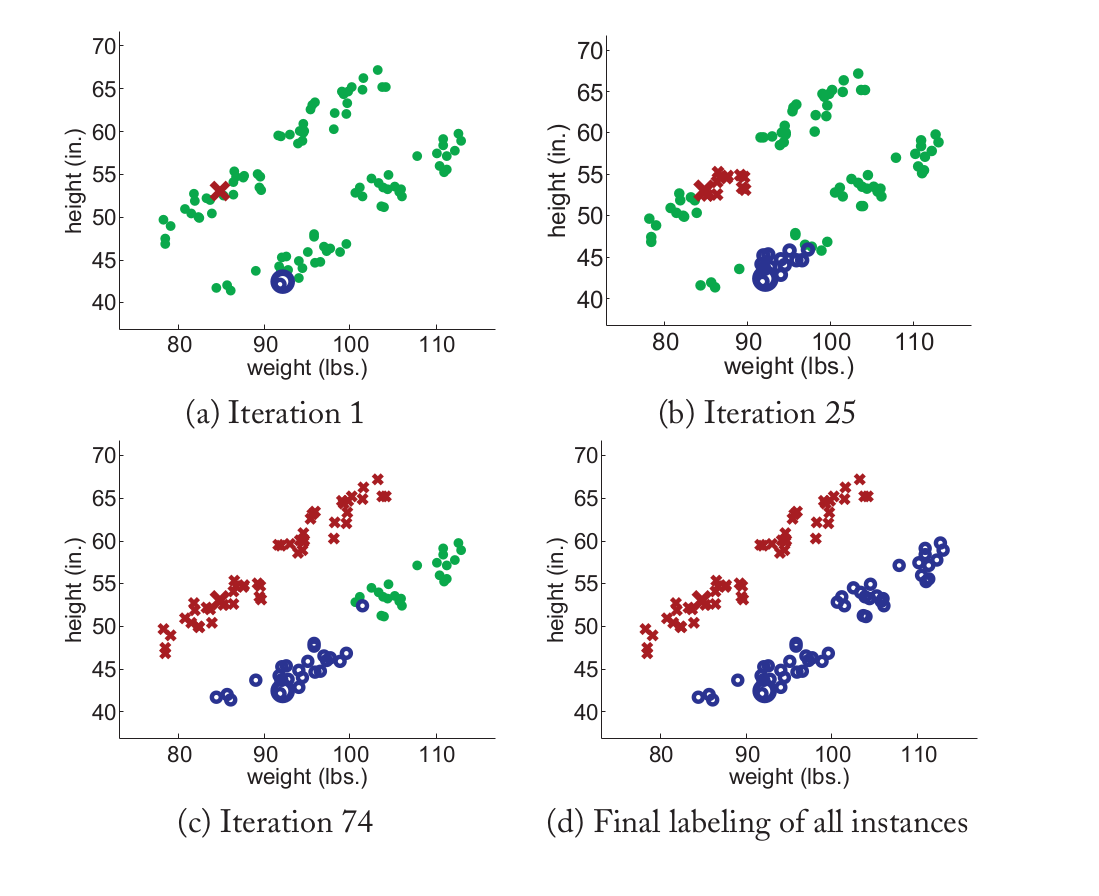
\includegraphics[width=\linewidth]{asset/image/semisupervised.png}
                  \caption{Quá trình dự đoán của mô hình 1-nearest-neighbor với 100 điểm chưa gán nhãn màu xanh (green). }
                  \label{fig:semi1}
              \end{center}
          \end{figure}

    \item Học tăng cường (reinforcement learning)

          Phương pháp học tăng cường là một dạng khác biệt hoàn toàn với các phương pháp đã được liệt kê. Một cách chung nhất, phương pháp này thay vì tập trung vào dữ liệu thì việc học được tiến hành bằng cách tương tác trực tiếp với môi trường (environment) theo hình thức thử sai (trial-and-error). Trong học tăng cường, một khái niệm quan trọng là agent, tức là mô hình chúng ta được coi như là một thực thể, tự vận động cải thiện. Mỗi lần muốn tương tác với môi trường, agent thực hiện một hành động (action) và thu về một giá trị phần thưởng (reward). Nhiệm vụ của agent là học cách để tương tác với môi trường sao cho reward nhận được là lớn nhất có thể, hay nói cách khác tìm ra  một policy tốt nhất. Hiện nay ứng dụng dễ  thấy nhất của học tăng cường là ở lĩnh vực game, với các sản phẩm nổi tiếng như AlphaGo, AlphaZero, AlphaStar đã chiến thắng các tuyển thủ thế giới trong những có chơi như cờ vây, StarCraft.

          \begin{figure}[t]
              \begin{center}
                  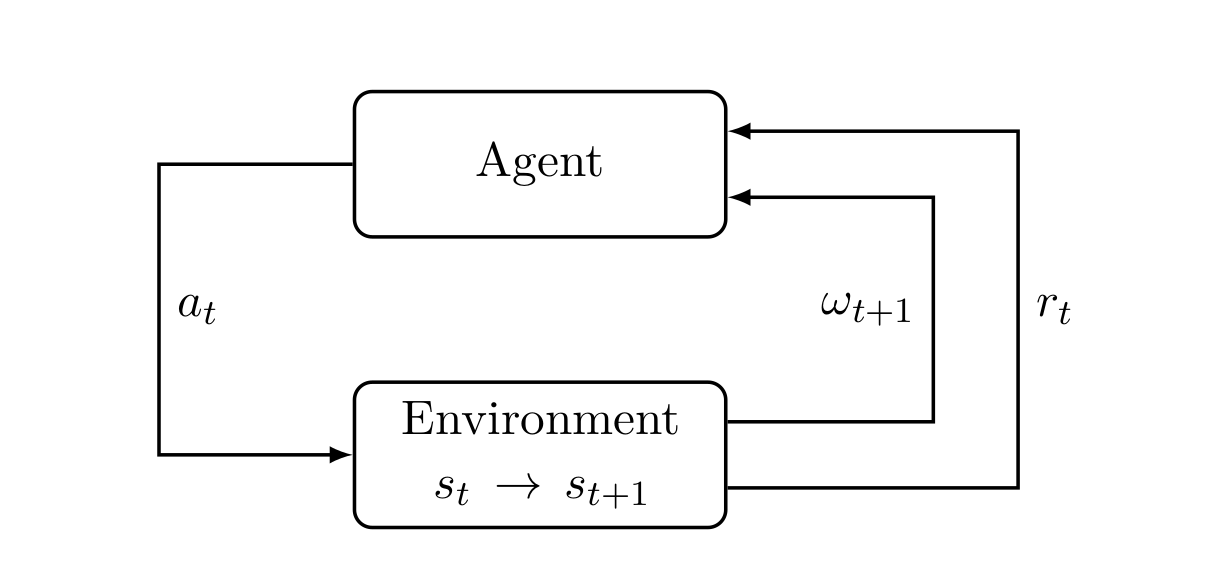
\includegraphics[width=\linewidth]{asset/image/rl.png}
                  \caption{Tương tác agent-environment trong học tăng cường (tham khảo \cite{franccois2018introduction}). }
                  \label{fig:semi2}
              \end{center}
          \end{figure}
\end{enumerate}

% \textbf{Phân loại theo ứng dụng}

% \begin{enumerate}
%     \item Phân loại (classification)
%     \item Hồi quy (regression)
%     \item 
% \end{enumerate}
